% University/School Laboratory Report
% LaTeX Template
% Version 3.1 (25/3/14)
%
% This template has been downloaded from:
% http://www.LaTeXTemplates.com
%
% Original author:
% Linux and Unix Users Group at Virginia Tech Wiki 
% (https://vtluug.org/wiki/Example_LaTeX_chem_lab_report)
%
% License:
% CC BY-NC-SA 3.0 (http://creativecommons.org/licenses/by-nc-sa/3.0/)
%

%	packages and such!

\documentclass{article}

\usepackage{mathptmx} % math functions!
\usepackage{amsmath} % moar math

\usepackage[11pt]{moresize} % different letters sizes
\usepackage{float} % enables accurate location of tables

\usepackage[utf8]{inputenc} % so you can type accented letters

\usepackage{caption} % to make personalized captions

\usepackage{graphicx} % required for the inclusion of images

\setlength{\parindent}{1cm} % paragraph indenting


\title{P\^endulo Composto \\ Experimento 1} % main title
\author{F 229 \\ \textsc{Grupo 1}}
\date{17 de Setembro, 2014}


\begin{document} % actually starts the document here
\maketitle

% members of the group
\begin{center}
	\begin{tabular}{l r l}
		Integrantes: & Henrique Noronha Facioli & 157986 \\
		& Guilherme Lucas da Silva & 155618 \\
		& Beatriz Sechin Zazulla & 154779 \\
		& Lucas Alves Racoci & 156331 \\
		& Isadora Sophia Garcia Rodopoulos & 158018 \\
	\end{tabular}
\end{center}


\section{Resumo}
Neste experimento, estudamos o funcionamento e as equações que regem o movimento de um pêndulo composto de duas barras, consideradas homogêneas. Valendo-nos da lei que descreve o período de um pêndulo para pequenas amplitudes de oscilação, $T = \sqrt{ \cfrac { D + \frac{ k^2\ } {D} } {g} }$, fomos capazes de determinar, com seus respectivos erros, a aceleração da gravidade ($g$), o raio de giração ($k$) e o momento de inércia no referencial do centro de massa ($I_{CM} = M \times k^2$, onde $M$ é a massa total) do sistema. 

Medimos, para tal, variações de $T$ em função de $D$ (distância do ponto de suspensão ao $CM$ do pêndulo) com o auxilio de um photogate ligado a um cronômetro inteligente, e formulamos um gráfico linearizado da equação acima, tomando os eixos por $T^2D \times D^2$ em função de $D^2$. 


\section{Objetivo}
O objetivo desse experimento foi analisar o movimento de um pêndulo composto, a partir de diferentes centros de massa obtidos nas diversas posições das quais o objeto de estudo foi posicionado no eixo de suspensão.

Além disso, a experiência desejava determinar o raio de giração e o momento de inércia em relação ao centro de massa e, também, a gravidade. Todos com seus respectivos erros.


\section{Procedimentos e coleta de dados}

Foi necessário os seguintes materiais para a execução do experimento:
\begin{enumerate} 
	\item Pêndulo composto; 
	\item Eixo de suspensão; 
	\item Régua de 1 $m$; 
	\item Balança de precisão;
	\item Cronômetro inteligente com \textit{photogate}.
 \end {enumerate} 

Para iniciá-lo, medimos o tamanho e a massa das duas barras que compõem o pêndulo, para posterior obtenção do centro de massa do sistema. A cada diferente posição que o pêndulo foi colocado no eixo de suspensão medimos a distância $D$ entre o centro de massa e a posição que o mesmo estava e acertamos o cronômetro com o \textit{photogate} para o modo pêndulo, no qual, após alguns instantes, nos era retornado o período $T$ do objeto de estudo.

Então, foi possível construir um gráfico T$^2$D $\times$  D$^2$ para a obtenção dos parâmetros objetivados. Tomamos alguns cuidados para o sucesso do experimento, entre eles: manter o ângulo de lançamento próximos a 15$^{\circ}$  e o feixe do \textit{photogate} estar perpendicular a trajetória do pêndulo.

\begin{table}[!ht]
	\begin{center}
		\caption*{\textbf{Tabela 1:} Medidas referentes às duas barras com o parafuso}
		\begin{tabular}{| l | l |}
			\cline{2-2} \multicolumn{0}{c|}{ } & \multicolumn{1}{c|}{\textbf{Massa ($Kg$)}} \\  \cline{1-2}
			\multicolumn{0}{|c|}{\textbf{Medida}} & 1,2790\\ \hline
			\multicolumn{0}{|c|}{\textbf{Erro Instrumental}} & 0,0001\\ \hline
		\end{tabular}
	\end{center}
\end{table}

\begin{table}[!ht]
	\begin{center}
		\caption*{\textbf{Tabela 2:} Medidas referentes à barra maior}
		\begin{tabular}{| c | c | c | c |}
			\cline{2-4} \multicolumn{0}{c|}{ } & \multicolumn{1}{c|}{\textbf{Massa ($Kg$)}} & \multicolumn{1}{c|}{\textbf{Comprimento ($m$)}} & \multicolumn{1}{c|}{\textbf{Largura ($m$)}}  \\  \cline{1-4}
			\multicolumn{0}{|c|}{\textbf{Medida}} & 0,9038 & 1,4830 & 0,0390\\ \hline
			\multicolumn{0}{|c|}{\textbf{Erro Instrumental}} & 0,0001 & 0,0005 & 0,0005\\ \hline
		\end{tabular}
	\end{center}
\end{table}

\begin{table}[!ht]
	\begin{center}
		\caption*{\textbf{Tabela 3:} Medidas referentes à barra menor}
		\begin{tabular}{| c | c | c | c |}
			\cline{2-4} \multicolumn{0}{c|}{ } & \multicolumn{1}{c|}{\textbf{Massa ($Kg$)}} & \multicolumn{1}{c|}{\textbf{Comprimento ($m$)}} & \multicolumn{1}{c|}{\textbf{Largura ($m$)}}  \\  \cline{1-4}
			\multicolumn{0}{|c|}{\textbf{Medida}} & 0,3752 & 0,1610 & 0,0380\\ \hline
			\multicolumn{0}{|c|}{\textbf{Erro Instrumental}} & 0,0001 & 0,0005 & 0,0005\\ \hline
		\end{tabular}
	\end{center}
\end{table}

\afterpage {\clearpage}

\begin{table}[!ht]
	\begin{center}
		\caption*{\textbf{Tabela 4:} Resultado das medidas experimentais realizadas com o \textit{photogate}}
		\begin{tabular}{| c | c | c | c | c |}
			\hline  \multicolumn{1}{|c|}{\textbf{N}} & \multicolumn{1}{c|}{\textbf{T ($s$)}} & \multicolumn{1}{c|}{\textbf{$\sigma_T$ ($s$)}} & \multicolumn{1}{c|}{\textbf{R ($m$)}} & \multicolumn{1}{c|}{\textbf{$\sigma_R$ ($m$)}} \\  \hline
			\multicolumn{0}{|c|}{\textbf{1}} & 1,8888&0,0001&1,0361&0,0005 \\ \hline
			\multicolumn{0}{|c|}{\textbf{2}} & 1,8901&0,0001&0,9957&0,0005\\ \hline
			\multicolumn{0}{|c|}{\textbf{3}} & 1,9051&0,0001&0,9419&0,0005 \\ \hline
			\multicolumn{0}{|c|}{\textbf{4}} & 1,9369&0,0001&0,8923&0,0005\\ \hline
			\multicolumn{0}{|c|}{\textbf{5}} & 1,9925&0,0001&0,8418&0,0005 \\ \hline
			\multicolumn{0}{|c|}{\textbf{6}} & 2,0914&0,0001&0,7928&0,0005 \\ \hline
		\end{tabular}
		\caption*{

		Em que $T$ é o período do pêndulo, $R$ é a medida do centro de rotação até a origem e $N$ corresponde ao número de medidas.}
	\end{center}
\end{table}


\begin{table}[!ht]
	\begin{center}
		\caption*{\textbf{Tabela 5:} Valores do $CM$ medido experimentalmente e calculado}
		\begin{tabular}{| c | c |}
			\hline 
			\multicolumn{0}{|c|}{\textbf{$X_{CM}$ \textsc{Experimental}} ($m$)} & 0,5550 \\ \hline
			\multicolumn{0}{|c|}{\textbf{$\sigma_{X_{CM} \textsc{Experimental}}$} ($m$)} & 0,0007 \\ \hline
			\multicolumn{0}{|c|}{\textbf{$X_{CM}$ \textsc{Calculado}} ($m$)} & 0,5508 \\ \hline
			\multicolumn{0}{|c|}{\textbf{$\sigma_{X_{CM} \textsc{Calculado}}$} ($m$)} & 0,0002 \\ \hline
		\end{tabular}
	\end{center}
\end{table}

\begin{table}[!ht]
	\begin{center}
		\caption*{\textbf{Tabela 6:} Distâncias utilizadas a partir do $CM$ experimental e calculado}
		\begin{tabular}{| c | c | c | c | c |}
			\hline  \multicolumn{1}{|c}{\textbf{N}} & \multicolumn{1}{|c|}{\textbf{D ($X_{CM}$ \textsc{Exp})} ($m$)} & \multicolumn{1}{c|}{\textbf{$\sigma_{D (X_{CM} \textsc{Exp})}$} ($m$)} & \multicolumn{1}{c|}{\textbf{D ($X_{CM}$ \textsc{Calculado})} ($m$)} & \multicolumn{1}{c|}{\textbf{$\sigma_{D (X_{CM} \textsc{Calculado})}$} ($m$)} \\  \hline
			\multicolumn{0}{|c|}{\textbf{1}} &0,48&0,01&0,4852&0,0004\\ \hline
			\multicolumn{0}{|c|}{\textbf{2}} & 0,44&0,01&0,4442&0,0004 \\ \hline
			\multicolumn{0}{|c|}{\textbf{3}} & 0,39&0,01&0,3902&0,0004 \\ \hline
			\multicolumn{0}{|c|}{\textbf{4}} &0,34&0,01&0,3412&0,0004 \\ \hline
			\multicolumn{0}{|c|}{\textbf{5}} &0,29&0,01&0,2902&0,0003\\ \hline
			\multicolumn{0}{|c|}{\textbf{6}} &0,24&0,01&0,2412&0,0003\\ \hline
		\end{tabular}
	\end{center}
\end{table}

\afterpage{\clearpage}

\begin{table}[!ht]
	\begin{center}
		\caption*{\textbf{Tabela 7:} Valores de $T^2D \times D^2$ com seus respectivos erros, a partir do $CM$ experimental}
		\begin{tabular}{| c | c | c | c | c |}
			\hline  \multicolumn{1}{|c|}{\textbf{N}} & \multicolumn{1}{c|}{\textbf{D$^2$ ($m^2$)}} & \multicolumn{1}{c|}{\textbf{$\sigma_{D^2}$ ($m^2$)}} & \multicolumn{1}{c|}{\textbf{T$^2$D ($s^2m$)}} & \multicolumn{1}{c|}{\textbf{$\sigma_{T^2D}$ ($s^2m$)}} \\  \hline
			\multicolumn{0}{|c|}{\textbf{1}} &0,2314&0,0070&1,72&0,03 \\ \hline
			\multicolumn{0}{|c|}{\textbf{2}} & 0,1936&0,0061&1,57&0,03 \\ \hline
			\multicolumn{0}{|c|}{\textbf{3}} & 0,1490&0,0051&1,40&0,03 \\ \hline
			\multicolumn{0}{|c|}{\textbf{4}} &0,1136&0,0042&1,26&0,02\\ \hline
			\multicolumn{0}{|c|}{\textbf{5}}&0,0818&0,0034&1,14&0,02 \\ \hline
			\multicolumn{0}{|c|}{\textbf{6}}&0,0562&0,0026&1,04&0,02 \\ \hline
		\end{tabular}
	\end{center}
\end{table}

\begin{table}[!ht]
	\begin{center}
		\caption*{\textbf{Tabela 8:} Valores de $T^2D \times D^2$ com seus respectivos erros, a partir do $CM$ calculado}
		\begin{tabular}{| c | c | c | c | c |}
			\hline  \multicolumn{1}{|c|}{\textbf{N}} & \multicolumn{1}{c|}{\textbf{D$^2$ ($m^2$)}} & \multicolumn{1}{c|}{\textbf{$\sigma_{D^2}$ ($m^2$)}} & \multicolumn{1}{c|}{\textbf{T$^2$D ($s^2m$)}} & \multicolumn{1}{c|}{\textbf{$\sigma_{T^2D}$ ($s^2m$)}} \\  \hline
			\multicolumn{0}{|c|}{\textbf{1}} &0,2354&0,0004&1,731&0,002\\ \hline
			\multicolumn{0}{|c|}{\textbf{2}} & 0,1973&0,0003&1,587&0,001 \\ \hline
			\multicolumn{0}{|c|}{\textbf{3}} & 0,1522&0,0003&1,416&0,001\\ \hline
			\multicolumn{0}{|c|}{\textbf{4}} & 0,1164&0,0002&1,280&0,001 \\ \hline
			\multicolumn{0}{|c|}{\textbf{5}} & 0,0842&0,0002&1,152&0,001\\ \hline
			\multicolumn{0}{|c|}{\textbf{6}} & 0,0582&0,0002&1,055&0,002\\ \hline
		\end{tabular}
		\caption*{

		Em que $D$ é a distância entre o centro de massa do sistema e o ponto de suspensão.}
	\end{center}
\end{table}


\section{Análise dos resultados}

Na tentativa de avaliar as possíveis consequências de cada método utilizamos duas vias de obtenção do centro de massa do sistema pêndulo composto de duas barras. 

A primeira foi o cálculo da média ponderada pelas massas dos centros de massa de cada barra em relação a uma origem estabelecida consideramos as barras homogêneas (cada qual com seu suposto centro de massa no seu centro geométrico).

\begin {center}
{\large $X_{CM}= \cfrac{(m_1 \times \frac{l_1}{2}+ m_2 \times (\frac{l_2}{2} +d_{12}))}{m_1+m_2}$} \\
\end {center}

Onde: 
\begin{itemize} 
	\item \textbf{1} é a maior barra e \textbf{2} é a menor;
	\item $l_n$ é o comprimento da barra n;
	\item $m_n$ é a massa da barra n;
	\item $d_{12}$ é a distância entre as extremidades próximas a origem da barra 1 e a barra 2
\end {itemize}

A segunda via utilizada foi a obtenção experimental do centro de massa, através do equilíbrio do sistema composto pelas duas massas sobre um ponto no qual a barra não girava, permanecendo na horizontal. Ambos os valores e erros estão especificados na tabela 5.

Com o centro de massa definido, é possível calcular $D$ (tabela 6) e desenvolver os dados necessários para a confecção dos gráficos (tabela 7 e 8). Após a realização dos cálculos e a confecção dos gráficos, um para cada caminho, pudemos identificar que ambas as modalidades geraram valores satisfatórios ($g = 10,33 \cfrac{m}{s^2}$, $I_{CM} = 1,8 Kg\times m^2$, $k = 1,2 m$ para valores advindos do cálculo do centro de massa, e $g = 10,2 \cfrac{m}{s^2}$, $I_{CM} = 1,7 Kg\times m^2$, $k = 1,2 m$ para valores advindos da tomada experimental do CM). Entretanto, percebemos algumas divergências relacionadas aos erros associados a alguns desses valores. 

No caso da medição experimental do centro de massa, o erro associado à acelera-ção da gravidade ($g$) foi satisfatório, $\sigma_g = 0,5 \cfrac{m}{s^2}$, mostrando que o valor de 9,8 $\cfrac{m}{s^2}$ está presente na faixa dada. Já no caso do cálculo do centro de massa, o erro associado ($\sigma_g = 0,03 \cfrac{m}{s^2}$) não permitiu que o valor ideal ocupasse tal faixa.

Deste modo, concluímos que a consideração da homogeneidade das barras pode ter sido a causa da disparidade, apontando para um erro em tal avaliação.
Outras possíveis fontes de erro incluem: 

\begin{itemize} 
	\item O atrito entre o eixo de rotação e a barra;
	\item A realização de uma única medida com o cronometro, o que elimina o erro estatístico, que poderia ser suficiente para conter o valor esperado para $g$.
\end {itemize}

O resultado dos cálculos realizados e as grandezas requisitadas podem ser encontrados resumidamente nas tabelas e gráficos a seguir:

\begin{table}[!ht]
	\begin{center}
		\caption*{\textbf{Tabela 9:} Valores referentes ao Método dos Mínimos Quadrados a partir dos dados experimentais}
		\begin{tabular}{| c | c | c | c | c | c |}
			\hline  \multicolumn{1}{|c|}{\textbf{N}} & \multicolumn{1}{c|}{\textbf{W}} & \multicolumn{1}{c|}{\textbf{WX}} & \multicolumn{1}{c|}{\textbf{WX$^2$}} & \multicolumn{1}{c|}{WXY} & \multicolumn{1}{c|}{WY} \\  \hline
			\multicolumn{0}{|c|}{\textbf{1}} & 1184,512605&274,0500207&63,40448684&470,2695551&2032,622417 \\ \hline
			\multicolumn{0}{|c|}{\textbf{2}} &1325,323484&256,5826266&49,6743965&403,3197481&2083,263162 \\ \hline
			\multicolumn{0}{|c|}{\textbf{3}} &1500,210542&223,52537&33,30438603&313,148028&2101,721039 \\ \hline
			\multicolumn{0}{|c|}{\textbf{4}} &1622,363984&184,2502553&20,92511724&232,944466&2051,127209 \\ \hline
			\multicolumn{0}{|c|}{\textbf{5}} & 1687,569685&138,0364499&11,29082946&156,7315666&1916,12752 \\ \hline
			\multicolumn{0}{|c|}{\textbf{6}} &1613,482124&90,62767744&5,090466014&93,9471054&1672,579277 \\ \hline
			\multicolumn{0}{|c|}{\textbf{S}}&8933,462424&1167,0724&183,6896821&1670,360469&11857,44062\\ \hline
		\end{tabular}
	\end{center}
\end{table}

\begin{table}[!ht]
	\begin{center}
		\caption*{\textbf{Tabela 10:} Resultados de $a$ e $b$ após o MMQ dos dados experimentais}
		\begin{tabular}{| c | c |}
			\hline 
			\multicolumn{0}{|c|}{\textbf{a}} & 3,9 \\ \hline
			\multicolumn{0}{|c|}{\textbf{$\sigma_a$}} & 0,2 \\ \hline
			\multicolumn{0}{|c|}{\textbf{b}} & 0,82\\ \hline
			\multicolumn{0}{|c|}{\textbf{$\sigma_b$}} & 0,03 \\ \hline
	\end{tabular}
	\end{center}
\end{table}

\begin{table}[!ht]
	\begin{center}
		\caption*{\textbf{Tabela 11:} Interpretação de $a$ e $b$ quanto a sua função teórica do pêndulo composto com os dados experimentais}
		\begin{tabular}{| c | c |}
			\hline 
			\multicolumn{0}{|c|}{\textbf{g ($\cfrac{m}{s^2}$)}} & 10,2 \\ \hline
			\multicolumn{0}{|c|}{\textbf{$\sigma_g$ ($\cfrac{m}{s^2}$)}} & 0,5 \\ \hline
			\multicolumn{0}{|c|}{\textbf{K ($m$)}} & 1,151 \\ \hline
			\multicolumn{0}{|c|}{\textbf{$\sigma_K$ ($m$)}} & 0,005 \\ \hline
			\multicolumn{0}{|c|}{\textbf{I ($Kg\times m^2$)}} & 1,70 \\ \hline
			\multicolumn{0}{|c|}{\textbf{$\sigma_I$ ($Kg\times m^2$)}} & 0,02 \\ \hline
		\end{tabular}
	\end{center}
\end{table}

\begin{figure}[!ht]
 	\centering
		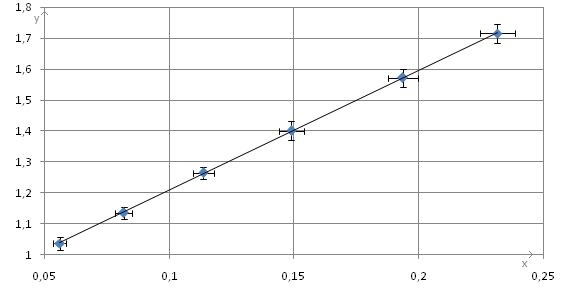
\includegraphics[width=0.9\textwidth]{experimentalmente}
	\caption*{\textbf{Figura 1:} Gráfico de $x$ = D$^2$ ($m^2$) $\times y$ =  T$^2$D ($s^2m$) considerando o centro de massa experimental}
\end{figure}

\afterpage{\clearpage}

\begin{table}[!ht]
	\begin{center}
		\caption*{\textbf{Tabela 12:} Valores referentes ao Método dos Mínimos Quadrados a partir dos dados calculados}
		\begin{tabular}{| c | c | c | c | c | c |}
			\hline  \multicolumn{1}{|c|}{\textbf{N}} & \multicolumn{1}{c|}{\textbf{W}} & \multicolumn{1}{c|}{\textbf{WX}} & \multicolumn{1}{c|}{\textbf{WX$^2$}} & \multicolumn{1}{c|}{WXY} & \multicolumn{1}{c|}{WY} \\  \hline
			\multicolumn{0}{|c|}{\textbf{1}} &436048,1243&102645,6608&24162,77263&177670,6246&754761,01\\ \hline
			\multicolumn{0}{|c|}{\textbf{2}} &467133,6579&92163,63341&18183,52238&146247,4714&741258,9297 \\ \hline
			\multicolumn{0}{|c|}{\textbf{3}} &496673,2139&75613,8297&11511,49505&107078,4404&703350,0794 \\ \hline
			\multicolumn{0}{|c|}{\textbf{4}} &504424,8206&58717,03745&6834,894609&75155,77838&645646,3349\\ \hline
			\multicolumn{0}{|c|}{\textbf{5}} &488141,0498&41103,70205&3461,119123&47352,77152&562354,0083 \\ \hline
			\multicolumn{0}{|c|}{\textbf{6}} &432174,8976&25138,70536&1462,265649&26519,10117&455906,1284 \\ \hline
			\multicolumn{0}{|c|}{\textbf{S}}&2824595,764&395382,5688&65616,06944&580024,1875&3863276,491\\ \hline
		\end{tabular}
	\end{center}
\end{table}

\begin{table}[!ht]
	\begin{center}
		\caption*{\textbf{Tabela 13:} Resultados de $a$ e $b$ após o MMQ dos dados calculados}
		\begin{tabular}{| c | c |}
			\hline 
			\multicolumn{0}{|c|}{\textbf{a}} & 3,82 \\ \hline
			\multicolumn{0}{|c|}{\textbf{$\sigma_a$}} & 0,01 \\ \hline
			\multicolumn{0}{|c|}{\textbf{b}} & 0,833\\ \hline
			\multicolumn{0}{|c|}{\textbf{$\sigma_b$}} & 0,002 \\ \hline
		\end{tabular}
	\end{center}
\end{table}

\begin{table}[!ht]
	\begin{center}
		\caption*{\textbf{Tabela 14:} Interpretação de $a$ e $b$ quanto a sua função teórica do pêndulo composto com os dados calculados}
		\begin{tabular}{| c | c |}
			\hline 
			\multicolumn{0}{|c|}{\textbf{g ($\cfrac{m}{s^2}$)}} & 10,33 \\ \hline
			\multicolumn{0}{|c|}{\textbf{$\sigma_g$ ($\cfrac{m}{s^2}$)}} & 0,03 \\ \hline
			\multicolumn{0}{|c|}{\textbf{K ($m$)}} & 1,1702 \\ \hline
			\multicolumn{0}{|c|}{\textbf{$\sigma_K$ ($m$)}} & 0,0003 \\ \hline
			\multicolumn{0}{|c|}{\textbf{I ($Kg\times m^2$)}} & 1,7514\\ \hline
			\multicolumn{0}{|c|}{\textbf{$\sigma_I$ ($Kg\times m^2$)}} & 0,0009 \\ \hline
		\end{tabular}
	\end{center}
\end{table}

\afterpage{\clearpage}

\begin{figure}[!ht]
 	\centering
		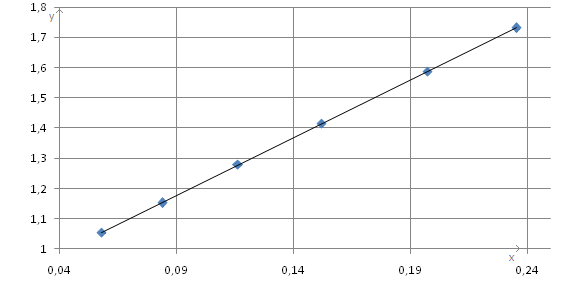
\includegraphics[width=0.95\textwidth]{calculado}
	\caption*{\textbf{Figura 2:} Gráfico de $x$ = D$^2$ ($m^2$) $\times y$ =  T$^2$D ($s^2m$) considerando o centro de massa calculado}
\end{figure}


\section{Conclusão}

Foi possível concluir, ao final desse experimento, que o pêndulo composto testado apresentou comportamento dentro do esperado, o que significa dizer que a equação do período de um pêndulo para oscilações de pequena amplitude mostrou-se eficiente no contexto e da forma como realizamos o experimento. 

Portanto, apesar de o valor esperado, 9,8$\frac{m}{s^2}$, não ter sido obtido no cálculo que usou o centro de massa calculado considerando-se as barras homogêneas, o experimento foi bem sucedido em um panorama geral, pois ao usarmos uma margem de erro razoável, com o método de equilibrar a barra, o valor aparece obtida.


\end{document}